\graphicspath{{lectures/04_eloadas_abrak/}}

\section{4. előadás -- Picard--Lindelöf-tétel, folytathatóság és szétválasztható egyenletek}

\subsection{Picard--Lindelöf-tétel}

\noindent\textbf{Tétel (Picard--Lindelöf).}
Legyen $n\in\mathbb N$, $D\subseteq\mathbb R\times\mathbb R^n$ tartomány,
$f:D\to\mathbb R^n$ függvény, és tegyük fel, hogy
\begin{enumerate}[label=\arabic*)]
\item $f\in C(D)$;
\item $\forall(\tau,\xi)\in D_f$ pontban $f$ a második változójában
      \textbf{lokális Lipschitz-feltételnek} tesz eleget, azaz
      \[
      \forall(\tau,\xi)\in D_f\ \exists K(\tau,\xi)\subseteq D_f\ \text{ környezet}\quad
      \exists L=L(\tau,\xi)>0:\quad
      \forall (t,u),(t,v)\in K(\tau,\xi),
      \]
      \[
      \|f(t,u)-f(t,v)\|\le L\,\|u-v\|.
      \]
\end{enumerate}
Ekkor
\[
\boxed{\forall(\tau,\xi)\in D_f:\quad
\begin{cases}
 x'=f\circ(\operatorname{id},x),\\
 x(\tau)=\xi
\end{cases}
\quad\text{lokálisan egyértelműen oldható meg.}}
\]
Következésképpen a 3. előadás tétele alapján
\textbf{globálisan is egyértelműen oldható meg}, és létezik teljes megoldás.

\subsubsection*{Bizonyításvázlat: Banach-féle fixponttétel}
Rögzítsünk egy tetszőleges $(\tau,\xi)\in D_f$ kezdeti adatot.
Válasszunk $a,b>0$ számokat, valamint a $(\tau,\xi)$ pont körül
$H\subseteq D_f$ kompakt téglalapot, amelyen az $f$ korlátos és a
második változóban az $L>0$ Lipschitz-konstans érvényes.
Jelöljük
\[
 M:=\max_{(t,u)\in H}\|f(t,u)\|,
 \qquad 0<\alpha<\min\!\left\{a,\frac{b}{M},\frac1L\right\}.
\]
\noindent\textit{A kézirat rövid jelölése: $M:=\max_H f$; vektorértékű függvénynél a fenti normás értelmezést használjuk. A $M=0$ eset külön kezelhető.}

\begin{center}
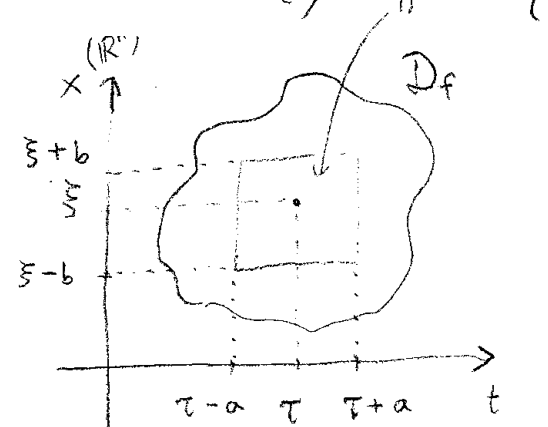
\includegraphics[width=.32\linewidth]{01_picard_teglalap.png}
\end{center}
\noindent Az eredeti ábrán $D_f$ a tartomány, $H$ a kompakt téglalap,
és a kezdőpont $(\tau,\xi)$.

A kezdetiérték-probléma és a vele ekvivalens integrálegyenlet:
\[
\begin{cases}
x'=f\circ(\operatorname{id},x),\\x(\tau)=\xi
\end{cases}
\quad\Longleftrightarrow\quad
x=\xi+\int_\tau^{\,\cdot} f\circ(\operatorname{id},x).
\]
Legyen
\[
\mathcal M:=\left\{\varphi\in
C\bigl([\tau-\alpha,\tau+\alpha],\mathbb R^n\bigr):
\ \varphi(\tau)=\xi,\quad \|\varphi-\xi\|_\infty\le b\right\}.
\]
Ekkor $(\mathcal M,\|\cdot\|_\infty)$ teljes metrikus tér. Definiáljuk
az $A:\mathcal M\to\mathcal M$ operátort:
\[
A(\varphi)(t):=\xi+\int_\tau^t f\bigl(s,\varphi(s)\bigr)\,ds
\quad \bigl(t\in[\tau-\alpha,\tau+\alpha]\bigr).
\]
A becslés \textbf{minden} $\varphi_1,\varphi_2\in\mathcal M$ esetén:
\[
\begin{aligned}
\|A(\varphi_1)-A(\varphi_2)\|_\infty
&\le \alpha\,L\,\|\varphi_1-\varphi_2\|_\infty,\\[-1pt]
&\hspace{15mm}\alpha L<1.
\end{aligned}
\]
Tehát $A$ kontrakció. A \textbf{Banach-féle fixponttétel} alapján
$\exists!\,\varphi\in\mathcal M$ úgy, hogy
\[
A(\varphi)=\varphi,
\]
vagyis $\varphi$ az integrálegyenlet, ezért a k.é.p. egyetlen lokális
megoldása. \hfill$\square$

\subsubsection*{Megjegyzés: szukcesszív approximációs sorozat}
Induljunk ki $\varphi_0\equiv c$ konstans függvényből, majd $\forall n\in\mathbb N_0$ mellett legyen
\[
\boxed{\displaystyle
\varphi_{n+1}(t)=\xi+\int_\tau^t
 f\bigl(s,\varphi_n(s)\bigr)\,ds
\qquad\bigl(t\in I \bigr).}
\]
Ekkor a $(\varphi_n)_{n\in\mathbb N_0}$ sorozat \textbf{egyenletesen
konvergál} az $A$ operátor egyetlen fixpontjához; ez a k.é.p. közelítő
megoldását adja.

\subsection{A megoldások folytathatósága}

A létezési és egyértelműségi tételek \emph{lokálisak}: egy intervallumon
adnak választ a létezésre és az egyértelműségre. A kérdés az, hogy
\textbf{meddig folytathatók a megoldások}.
\emph{„ameddig csak lehet"}.

\begin{center}
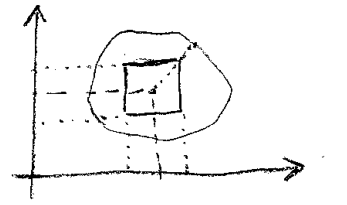
\includegraphics[width=.19\linewidth]{02_folytatas_kis_abra.png}
\end{center}

\subsubsection*{Definíció: határtól határig haladó megoldás}
Az $x'=f\circ(\operatorname{id},x)$, $x(\tau)=\xi$ k.é.p.
$\varphi$ megoldása \textbf{határtól határig halad}, ha
\[
\boxed{\begin{gathered}
\forall Q\subseteq D_f\ \bigl(Q\text{ kompakt}\bigr)\quad
\exists t_1,t_2\in D_\varphi:\\
 t_2<\tau<t_1,\\
 \bigl(t_1,\varphi(t_1)\bigr)\notin Q
 \quad\text{és}\quad
 \bigl(t_2,\varphi(t_2)\bigr)\notin Q.
\end{gathered}}
\]

\begin{center}
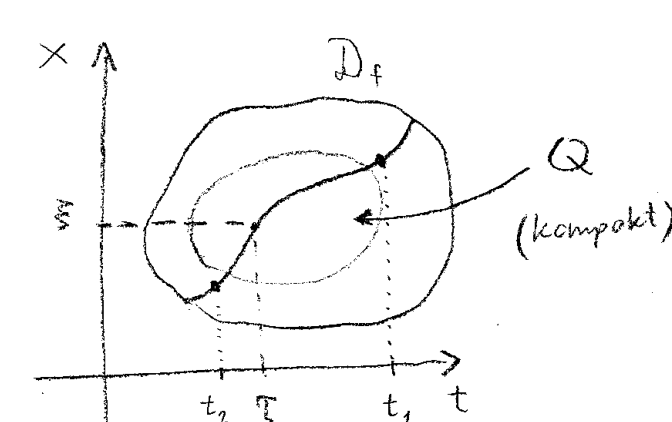
\includegraphics[width=.34\linewidth]{03_folytatas_tartomany.png}
\end{center}
\noindent Az eredeti ábrán a megoldásgörbe a kompakt $Q$ halmazt
mindkét időirányban elhagyja, miközben a $D_f$ tartományban halad.

\noindent\textbf{Tétel.}
A \textbf{Picard--Lindelöf-tétel feltételei mellett}
\[
\boxed{\forall(\tau,\xi)\in D_f\quad
\forall\varphi\text{ teljes megoldás}:\quad
\varphi\text{ határtól határig halad}.}
\]
\noindent\textbf{Bizonyítás:} Nélkül.

\subsection{A megoldások explicit előállítása}
\noindent\textbf{Megjegyzés.}
A kézirat kvadratúrával (integrálással) megoldható típusokra tér át;
utal a Kamke-könyvre, a Wolfram Alphára és a szimbolikus programcsomagokra.
A szétválasztható változójú egyenletekhez az
\emph{Analízis alkalmazásai, 5. előadás} segédanyagot is megadja.

\subsubsection*{1. Szétválasztható változójú differenciálegyenletek}
\noindent\textbf{Definíció.}
Legyenek $I,J\subseteq\mathbb R$ \textbf{nyílt intervallumok},
$\Omega:=I\times J$, továbbá
\[
 g:I\to\mathbb R,\qquad h:J\to\mathbb R
 \qquad\text{folytonos függvények.}
\]
Az
\[
\boxed{x'(t)=g(t)\,h(x(t))\quad\text{vagy röviden}\quad
x'=g\cdot(h\circ x)}
\]
egyenlet \textbf{szétválasztható változójú differenciálegyenlet}.
A hozzá tartozó k.é.p.:
\[
\boxed{\begin{cases}x'=g\cdot(h\circ x),\\x(\tau)=\xi,
\end{cases}
\qquad (\tau,\xi)\in I\times J.}
\]

\begin{center}
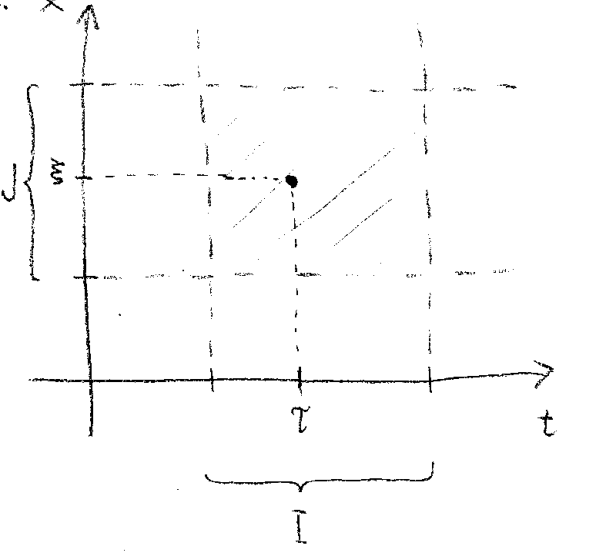
\includegraphics[width=.27\linewidth]{04_szetvalaszthato_tartomany.png}
\end{center}

\noindent\textbf{Levezetés.}
Legyen $U\subseteq I$ nyílt intervallum,
$\varphi:U\to J$ a k.é.p. megoldása, tehát
\[
 \forall t\in U:\quad
 \varphi'(t)=g(t)h(\varphi(t)),
 \qquad\varphi(\tau)=\xi.
\]
Tegyük fel, hogy $0\notin\mathcal R_h$, ahol
$\mathcal R_h:=h(J)$ az $h$ értékkészlete.
Ekkor oszthatunk $h(\varphi(t))$-vel:
\[
\frac{\varphi'(t)}{h(\varphi(t))}=g(t).
\]
A láncszabály szerint
\[
\left(\left(\int\frac1h\right)\circ\varphi\right)'(t)=g(t),
\]
és a kezdeti feltételt felhasználva \textbf{implicit alakban}:
\[
\boxed{\forall t\in U:\qquad
\int_\xi^{\varphi(t)}\frac{1}{h(u)}\,du
=\int_\tau^t g(s)\,ds.}
\]
Mivel $h$ folytonos és $0\notin\mathcal R_h$, az $1/h$
állandó előjelű $J$-n, így
\[
 H(v):=\int_\xi^v\frac1{h(u)}\,du
\quad(v\in J)
\]
szigorúan monoton, ezért van inverze. A megoldás \textbf{explicit alakja}:
\[
\boxed{\displaystyle
\varphi(t)=
\left(\int_\xi^{\,\cdot}\frac1h\right)^{-1}
\!\left(\int_\tau^t g(s)\,ds\right).}\tag{$*$}
\]
Kérdés, hogy a $(*)$ képlet \textbf{melyik legbővebb intervallumon}
értelmezhető. Az inverz értelmezési tartományához
\[
\boxed{\inf_{u\in J}\int_\xi^u\frac1{h(v)}\,dv
\quad<\quad \int_\tau^t g(s)\,ds
\quad<\quad
\sup_{u\in J}\int_\xi^u\frac1{h(v)}\,dv}
\]
szükséges.

\subsubsection*{Tétel: a szétválasztható k.é.p. megoldása}
\noindent\textbf{Tétel.}
Legyen $I,J\subseteq\mathbb R$ nyílt intervallum, és
\begin{enumerate}[label=(\alph*)]
\item $g:I\to\mathbb R$ és $h:J\to\mathbb R$ folytonos függvények;
\item $0\notin\mathcal R_h$.
\end{enumerate}
Ekkor
\[
\boxed{\forall(\tau,\xi)\in I\times J:\quad
\begin{cases}
x'=g\cdot(h\circ x),\\x(\tau)=\xi
\end{cases}
\text{ globálisan egyértelműen oldható meg.}}
\]
Az $\widetilde\varphi$ \textbf{teljes megoldásra}
\[
\boxed{\forall t\in D_{\widetilde\varphi}:\quad
\int_\xi^{\widetilde\varphi(t)}\frac{1}{h(u)}\,du
=\int_\tau^t g(s)\,ds.}
\]
Legyen
\[
\boxed{\begin{aligned}
I^*:=\biggl\{t\in I:\quad
&\inf_{u\in J}\int_\xi^u\frac1{h(v)}\,dv
 <\int_\tau^t g(s)\,ds\\[-2pt]
&<\sup_{u\in J}\int_\xi^u\frac1{h(v)}\,dv
\biggr\}.
\end{aligned}}
\]
Ekkor $D_{\widetilde\varphi}$ az $I^*$ halmaznak a
\textbf{$\tau$-t tartalmazó legbővebb intervalluma}
(azaz összefüggő komponense).

\noindent\textbf{Megjegyzés.}
$I^*$ nyílt halmaz, mivel nyílt intervallumok egyesítése.
Az eredeti kézirat itt ér véget a \textbf{4. előadás} szempontjából;
a következő, 2019. 10. 09-i rész már az \textbf{5. előadás}.
